% Created 2018-05-17 Thu 19:22
\documentclass[a4paper,11pt]{article}
                % input
                \usepackage[utf8]{luainputenc}
                \usepackage{fontspec}
                \usepackage{unicode-math}
                \usepackage[novoc]{arabluatex}
                \newfontfamily\arabicfont[Script=Arabic]{Scheherazade}
                \newcommand{\arbt}[1]{{\Large{\arb{#1}}}} %{\arbt{...}}
                \newcommand{\arbT}[1]{{\LARGE\arb{#1}}} %\arbT{...}
                % layout
                \usepackage{layout}
                \usepackage{setspace} %package pour les interlignes
                \usepackage{multicol}
                \setlength{\columnsep}{40pt}
                \usepackage{xcolor} % package pour les couleurs
                % headers ...
                \usepackage{fancyhdr} % header etc
                \usepackage{fancybox} %package pour les encadrements supp
                \pagestyle{fancy} % Use en-tetes et des pieds de page personnaliser grâce fancyhdr
                \usepackage[Glenn]{fncychap}
                \fancyhead[L, R, C]{} % définition en-tête
                \fancyfoot[L, R]{} % définition pied de page
                \fancyfoot[C]{\thepage}
           		\renewcommand{\headrulewidth}{0pt} % ligne haut out
	        	\renewcommand{\footrulewidth}{0pt} % ligne bas out
                % others
                \usepackage{float}
                \usepackage{array, makecell} %pour les tableaux et makecell pour les cellules
                \usepackage{multirow} %pr tableau
                \newcolumntype{P}[1]{>{\centering\arraybackslash}m{#1}} %P{taille}
                % maths
                \usepackage{amsmath, amsthm} %package pour les maths
                \usepackage{lettrine}
                \usepackage{marvosym} %package de symbole
                % others
                \usepackage{wrapfig} % pour les capsules in text
                %defaut emacs packages
                \usepackage{fixltx2e}
                \usepackage{graphicx}
                \usepackage{longtable}
                \usepackage{float}
                \usepackage{wrapfig}
                \usepackage{rotating}
                \usepackage[normalem]{ulem}
                \usepackage{textcomp}
                \usepackage{wasysym}
                \usepackage{hyperref}
               

\usepackage[top=2cm, bottom=2cm, left=2cm, right=2cm]{geometry}
\author{Gueye Ousseynou\thanks{21505055}}
\date{\today}
\title{\textbf{Documentation devoir sur ontologie} \\ Cours de logique - S6}
\hypersetup{
  pdfkeywords={},
  pdfsubject={...},
  pdfcreator={...}}
\begin{document}

\maketitle
\setcounter{tocdepth}{3}
\tableofcontents

\section{Sujet}
\label{sec-1}

Il s'agit de créer une ontologie en rapport avec le sujet de la FCA à savoir la NBA.

\section{Description de l'ontologie}
\label{sec-2}

\subsection{Classe}
Pour les classes, nous avons :
\begin{itemize}
    \item \textbf{Conférence}
        \begin{itemize}
            \item {East}
            \item {West}
        \end{itemize}
    \item \textbf{Equipe}
    \item \textbf{Personne}
        \begin{itemize}
            \item HeadCoach
            \item Player \\
        \end{itemize}
\end{itemize}

Les trois classes en gras sont disjointes, de même que celles de même niveau.

\subsection{Propriétés}

Pour les propriétés, nous avons :
\begin{itemize}
    \item \textbf{isHeadCoachOf} 
    
    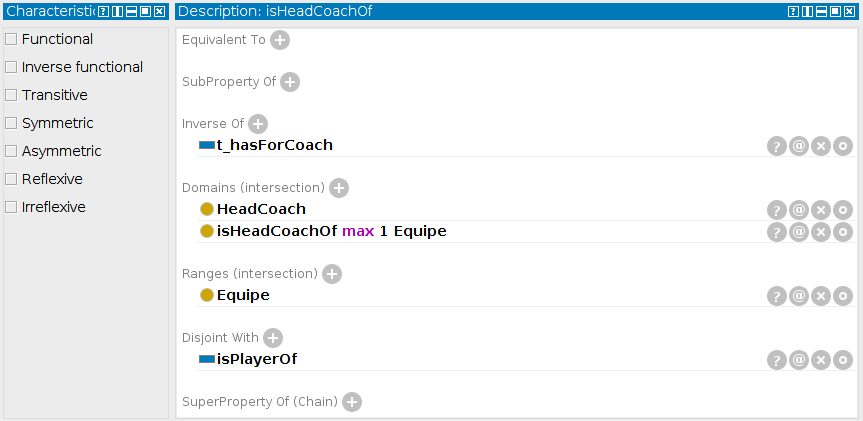
\includegraphics[width=.75\linewidth]{./img/1.png} \\
    
    \item \textbf{isPartOfConf}
    
    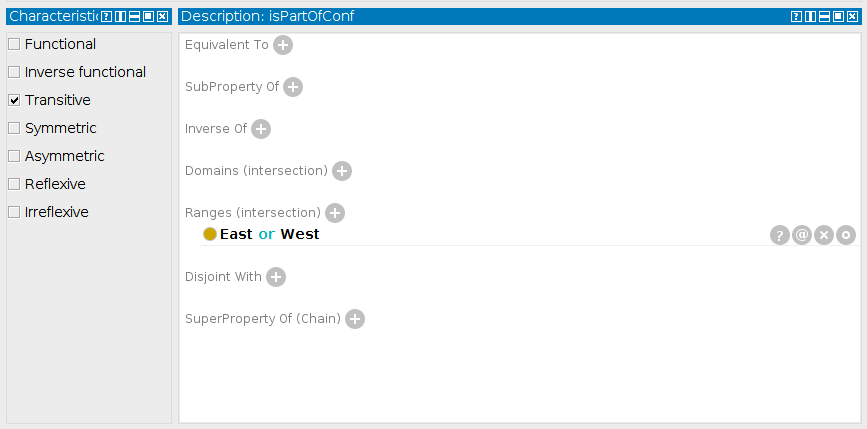
\includegraphics[width=.75\linewidth]{./img/2.png} \\
    
        \begin{itemize}
            \item isMemberOfDivEast \\
            
            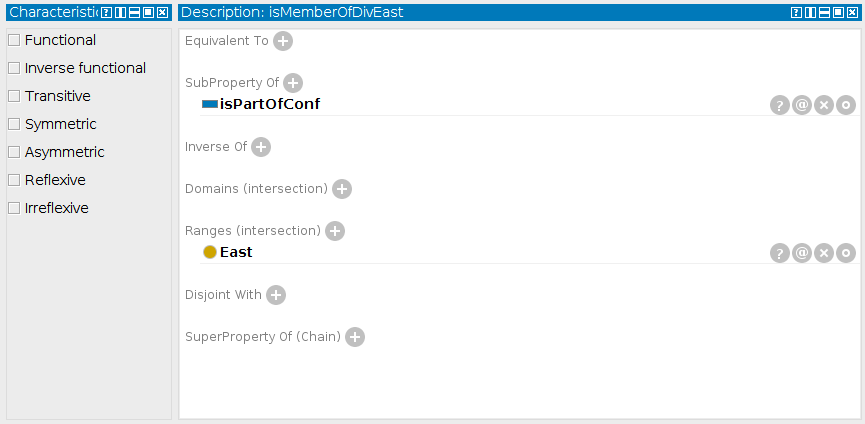
\includegraphics[width=.75\linewidth]{./img/3.png} \\
            
            \item isMemberOfDivWest \\
            
            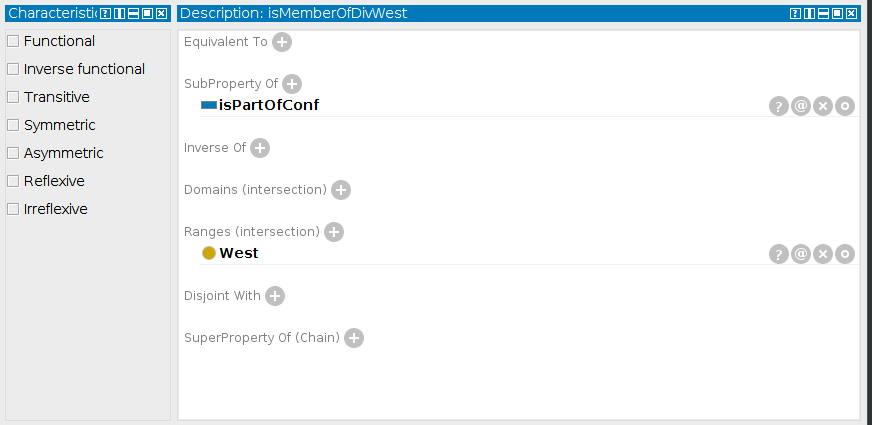
\includegraphics[width=.75\linewidth]{./img/4.png} \\
            
        \end{itemize}
        
    \item \textbf{isPlayerOf}
    
    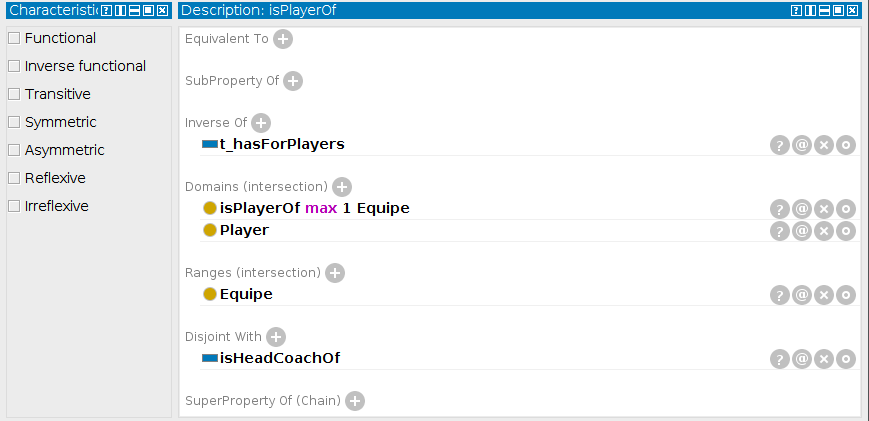
\includegraphics[width=.75\linewidth]{./img/5.png} \\
    
    \item \textbf{t\_hasForCoach}
    
    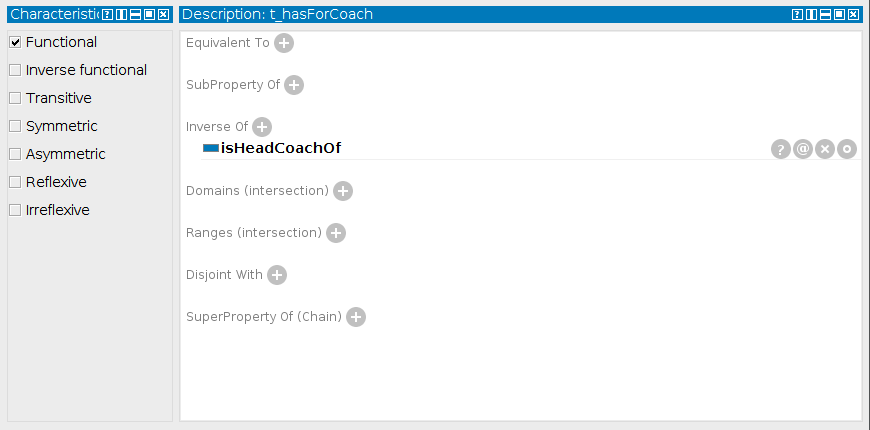
\includegraphics[width=.75\linewidth]{./img/6.png} \\
    
    \item \textbf{t\_hasForPlayers}
    
    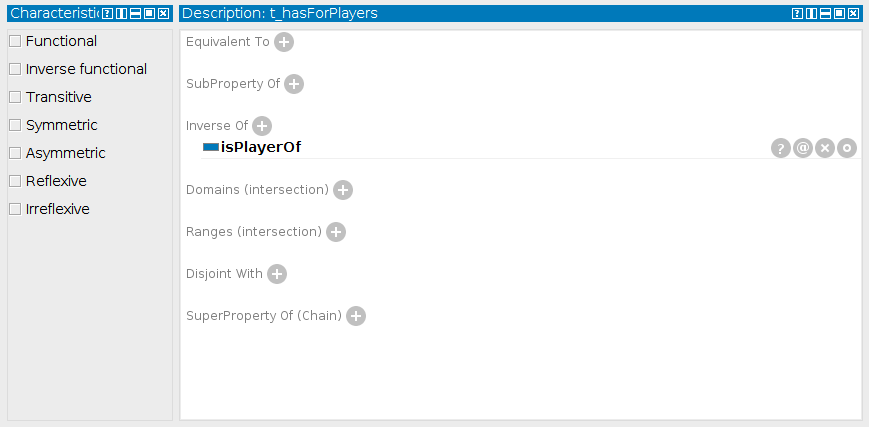
\includegraphics[width=.75\linewidth]{./img/7.png} \\
    
\end{itemize}

\subsection{Individus}

Pour les individus créés, et à juste à titre d'indication pour le lecteur, nous avons fait précéder les appelations par : \\
\begin{itemize}
    \item \textbf{conf} = conference (2).
    \item \textbf{d} = division (sous-partie d'une conférence) (6).
    \item \textbf{hc} = head coach (6).
    \item \textbf{p} = player (10).
    \item \textbf{t} = team (8). 
\end{itemize}

\section{Liaisons et résultats du reasoner}
\label{sec-3}

Notre but était, grâce aux propriétés, de donner pour chaque individu le minimum d'informations qui permette quand même au reasoner :

\begin{itemize}
    \item de trouver la classe des individus.
    \item de classer les individus comme instances de leur classe.
    \item de rajouter des propriétés si possible. \\
\end{itemize} 

Pour les reasonner, nous avons utiliser HermiT et Fact++. \\

La première, les reasonner ont détecté des incohérences que nous avons corrigées. \\

Désormais, chaque individu est bien classé de même que plusieurs propriétés sont justement rajoutées. \\


\section{Liens avec logique}
\label{sec-4}


$\forall x $ individu(x) $\rightarrow$ conference(x) $\vee$ equipe(x) $\vee$ personne(x)






% ...
\end{document}